% !TeX spellcheck = en_GB
\documentclass[10pt,a4paper,kul]{kulakarticle} %options: kul or kulak (default)

\usepackage[utf8]{inputenc}
\usepackage[english]{babel}
\usepackage[T1]{fontenc}
\date{2024 -- 2025}
\address{
	Engineering Technology\\
	Distributed Systems\\
	Bert Lagaise
}
\title{Report Final Project}
\author{Robbe Decapmaker, Wout Lyen, Lander Van Loock, Kobe Michiels}

\usepackage[backend=biber,style=ieee, natbib=true]{biblatex} % Use a proper package for managing bibliography
\addbibresource{ugh.bib}

\usepackage{hyperref}
\usepackage{graphicx}
\usepackage{amsmath, amssymb, amsthm}
\usepackage{siunitx}
\usepackage{flafter} 
\usepackage{pdfpages}
\usepackage{pgfplots}
\usepackage{caption}
\usepackage{subcaption}
\usepackage{multicol}
\usepackage{floatrow}
\usepackage{float}


\begin{document}
	\maketitle  
	\section*{Introduction}
		This report presents an overview of a modern web-based retail platform specializing in the sale of bicycles equipped with RGB LED strips, a product that blends functionality, safety, and aesthetic appeal for urban and recreational cyclists. The web-shop is designed to deliver a seamless shopping experience while leveraging a robust, distributed architecture deployed on Microsoft Azure.\\
		By operating across various administrative and geographic boundaries, the system ensures high availability, scalability, and resilience. The use of Azure’s global infrastructure enables efficient resource allocation, data redundancy, and compliance with regional data protection regulations. This report explores the technical design, deployment strategies, and operational considerations of the platform, with a focus on how distributed cloud services support the business’s scalability and cross-regional presence.

	\section{General Architecture}
		\begin{figure}[h]
			\centering
			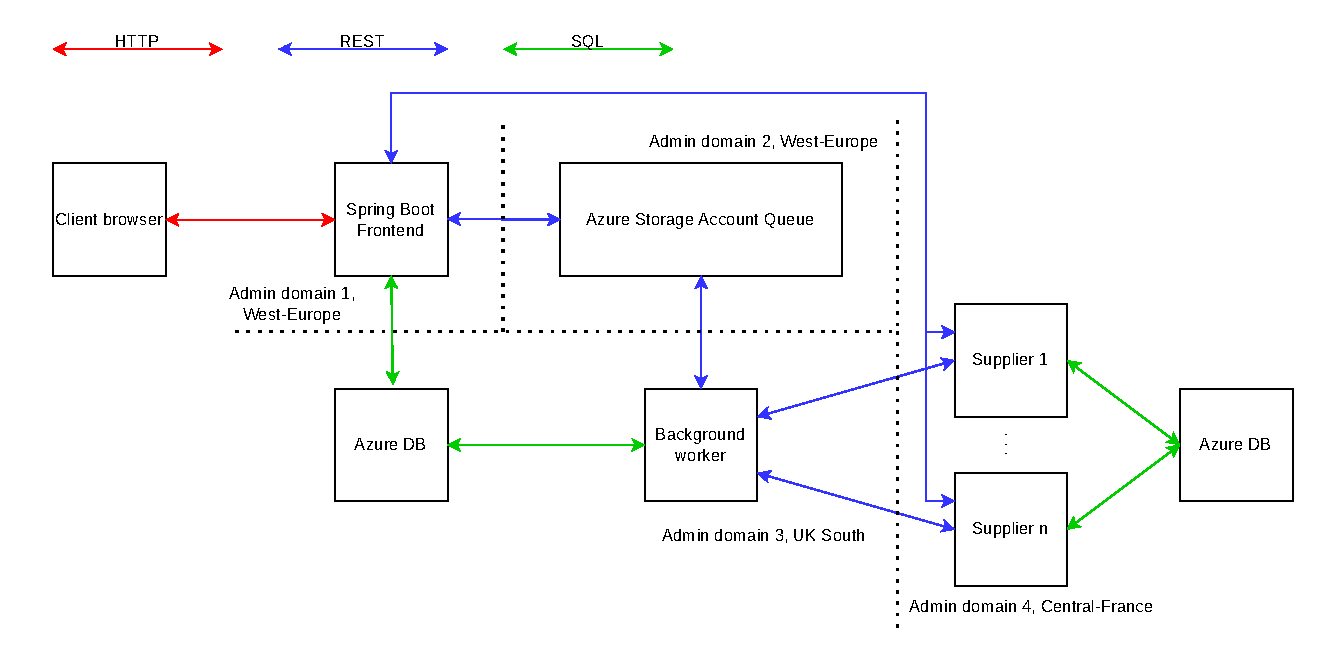
\includegraphics[width=1\linewidth]{images/arch}
			\caption{General overview of the architecture}
			\label{fig:arch}
		\end{figure}
		
	
	\section{Front-end Details}
	The Front-End makes it possible for the clients to order their products via our service and will transfer the order data to the broker for further processing.
	
	\subsection{Design}
	The front-end is build as a String Boot application using the Thymeleaf server-side Java template engine which allows HTML to be correctly displayed in browsers. It uses the Bootstrap open-source CSS framework and the Animate On Scroll (AOS) javascript library for adding animations to the website. The front-end makes uses of Auth0's Role-Based Access Control making it possible for clients to log in on the website. Every client gets the `User' role automatically assigned when logging in for the first time. There is also a `Manager' role available with which the clients that have that role can access pages that are not allowed to access for normal clients.\\
	\newline
	When a client with only the `User' role wants to access a page only accessible for clients with the `Manager' role will be blocked off by the security filter chain and will be welcomed with an 403 access-denied error message on the website stating that the client does not have permission to view the particular page. There are also web-pages implemented for the other common HTTP error codes (400, 404 \& 500) and a general error page when the error does within those error codes. The website has multiple endpoints of which some a publicly accessible, some only when the client has been logged in and some are only accessible when the logged in client has the `Manager' role. The different endpoints are:
	
	\begin{description}
		\item[/]: The home page showing some general information. (publicly accessible)
		\item[/products]: The products page which shows the products that are sold via our service sorted by suppier. (publicly accessible)
		\item[/profile]: The profile page which shows details of the user provided by Auth0 like the given and last name, roles, email, etc. (accessible after logging in)
		\item[/order/bicycle]: The first page of the order process where the client can choose which products he/she wants and the amount of every product from the bicycle supplier. (accessible after logging in)
		\item[/order/led \& /order/battery]: The following pages of the order process where the client can select products from the other two suppliers; which are the LED-Strip and Battery suppliers. (accessible after logging in)
		\item[/order/summary]: Gives a summary of all the selected products and provided the ability to actually order the produce when the client has selected some products or will show buttons to the different order pages so that the client can start ordering. (accessible after logging in)
		\item[/orders]: Gives a list of all the orders made by the client. It shows 18 orders per page and the client can go through the pages using the navigation buttons at the bottom of the website. (accessible after logging in)
		\item[/admin/orders]: Has the same functionality as the previous endpoint but now shows all the orders and the email address of the client of the order and is therefore only accessible after the client has logged in and has the `Manager' role assigned.
	\end{description}
	
	\noindent In the current implementation, the client does not need to provide a delivery address or payment information. However, this functionality can be easily added in the future when transitioning the system into a fully operational service. This could be achieved by introducing these fields on the `/order/summary' endpoint page, which the client would be required to fill in before placing an order. Currently, only logged-in clients are allowed to place orders. We use their email address to store the order, which enables clients with the `User' role to view their own order history.\\
	\newline
	When the client submits an order, the order data is stored in a SQL database, and the order ID is placed in an Azure Storage Queue. Both of these will be used by the broker to process the order, which will be discussed in more detail in the Broker Details subsection.\\
	\newline
	When a supplier is not available, the client can still order products from the other suppliers that are available while the website will show a notification on the order page of the specific not available supplier that the supplier is temporarily not available and a button to reload the page. When reloading the page, the selected items by the clients from the other available suppliers will still be selected as these are stored in a session attribute. Only when cancelling the order or actually submitting the order, this session attribute will be removed.
	
	\subsection{Deployment}
	The front-end is deployed as a Spring Boot application running on an Azure VM (1 vCore, 1GB RAM) located in West Europe. It communicates with the broker through an Azure Storage Queue that is also hosted on Azure, also located in West-Europe. This provides reliable asynchronous messaging. The database between the front-end and the broker is a SQL database hosted by Azure in UK-South.
	
	\section{Broker Details}
		The broker acts as a central orchestrator between the client application and the supplier system. 
		\subsection{Design}
		The broker is build as a Spring Boot application that is responsible for coordinating the distributed commit of client reservations across multiple supplier services. At the centre of its design is the Background Worker Java component that continuously polls an Azure Storage Queue every second for new messages. Every second, a total of 32 messages can be retrieved from the queue which  contain the corresponding ID's of client-side orders in the database that need to be processed.\\
		\newline
		To improve scalability and responsiveness, the Background Worker uses a multi-threaded executor that is configured to handle up to 8 concurrent threads. This allows simultaneous processing of multiple reservations. If necessary, there exists a task queue of up to 100 tasks so that messages retrieved from the queue can be processed right after each other instead of leaving threads waiting for the next message polling.\\
		\newline
		The orders are then processed using the distributed commit protocol. First, a UUID (unique reservation ID) is generated that will be used to identify orders in the communication between the broker and the suppliers. The broker then contacts the supplier's PHP endpoints to confirm the availability of the orders and to reserve them. This supplier PHP API will be covered in more detail in section \ref{ch:supplier-design} of this report. If all reservations are successful, the broker proceeds to invoke commit operations on each supplier. During the whole transaction, the status of the order is updated very accurately in the database. The used statuses are:
		
		\begin{description}
			\item[NEW]: the order is not retrieved yet from the queue by the broker.
			\item[PROCESSING]: the order is retrieved from the queue, a unique reservation ID is generated and assigned to the order.
			\item[RESERVING]: the unique reservation ID is successfully generated and stored in the database, starting reserving the order items with the suppliers.
			\item[RESERVED]: all items have been successfully reserved with the suppliers.
			\item[COMMITTING]: all items are being committed with the suppliers.
			\item[COMPLETED]: all items are committed with the suppliers and the order is completed successfully. There is no reverting back from here.
			\item[FAILED]: fatal failure in the order. This can be due to several reasons, but there is no retry after this and the order failed forever.
		\end{description}
		
		\noindent These detailed statuses have been made to improve the fault tolerance of the broker. If the broker fails somewhere, the message is left in the queue and retrieved again the next time the broker is going to process some messages. The status of the current order is then be retrieved, and if it was already in the middle of something, it will pick up from where it left. It is only when the order failed due to some fatal errors (e.g. incorrect message format, non-existent product in supplier, product not available with a supplier, etc.) that it is immediately removed from the queue because then a retry will lead to the same error. In addition, if a message has been retrieved more than 3 times from the queue, it will also be removed to prevent so-called "poison messages" which wander forever in the queue.\\
		\newline
		The order status can be queried by the suppliers at any time if they experience a network failure or for other reasons using a REST API endpoint. They will get the following status codes:
		 
		 \begin{description}
		 	\item[Code 0]: there is no decision yet.
		 	\item[Code 1]: the order is committed and completed.
		 	\item[Code 4]: the order failed, the reservation is aborted and a rollback message has been sent.
		 \end{description}
		
		\subsection{Deployment}
		The broker is deployed as a Spring Boot application running on an Azure VM (1 vCore, 1GB RAM) located in UK South. It communicates with the client side through an Azure Storage Queue that is also hosted on Azure, but located in West-Europe. This provides reliable asynchronous messaging. The database between the broker and the client application is a SQL database hosted by Azure in UK-South by another administration domain than the suppliers.
	
	\section{Supplier Details}
		Although the suppliers are an indirect part of the web-store, they do take part in the distributed commit. Because of this, careful thought had to be put in to ensure proper processing of an order. 
		\subsection{Design}\label{ch:supplier-design}
			A supplier is essentially a PHP API with a number of endpoints useful for retrieving information about products and orders. As well as making a distributed commit of-course. On a high level, the following endpoints are available:
			\begin{description}
				\item[list\_products] provides information such as id, name, description, stock and an image url for all products. 
				\item[reserve] provides a starting point for the distributed commit. It acts as a \emph{request} operation. It expects information such as a global order id, other partaking parties and of-course product information. 
				\item[show\_reserve] provides information about reservations currently filed by a user.
				\item[commit] provides a way to confirm a reservation. It acts as a\emph{commit} operation. It just needs to know which global order id needs to be committed. 
				\item[show\_commit] provides information about the commits currently filed by a user.
				\item[rollback\_reservation] provides a way to cancel a reservation. It acts as an \emph{abort} operation. It just needs to know which global order id needs to be reverted. 
				\item[rollback\_commit] provides a way to cancel a commit. It is not part of the standard two-phase commit but can be used for cancelling confirmed orders. 
				\item[cleanup\_reserve] provides a way for users with extra privileges to clean-up stale reservations in case they have been abandoned by the broker. 
				\item[transaction\_check] provides a way for users with extra privileges to request the status of any global order id, it acts as a part of the mechanism to communicate among suppliers in case of a broker failure. 
				\item[check\_other\_sup] provides a way for users with extra privileges to perform a synchronisation of waiting reservations with their respective peers.  
			\end{description}
			
			In order to secure these endpoints, we protected them with SSL so there would be no unencrypted data on the wire. This was done using free \emph{Let's Encrypt} certificates which renew automatically. Another level of protection is the API-keys which are required to talk to a supplier. These API keys are registered in a  database and are associated with an entity name and privilege level. This way, ordinary brokers can't perform the same tasks as an admin user. This helps to ensure critical actions such as clean-up and synchronisation are only performed by the right entity. Another layer of protection is the Nginx web-server which serves the PHP API to the outside world. It is configured to protect any assets which contain sensitive information, only allowing traffic to the PHP and picture assets. 
			
			In order to help avoid inconsistency in the suppliers, a lot of effort was put into making sure a malformed input has no effect on the transactions. This is done by checking the contents of a request to see if it contains the right data for performing the requested operation. Furthermore, if something does manage to slip through the cracks, the PHP works with DB transactions. Essentially, when a critical section of the code is reached, an SQL transaction is started. Following this, all operations are performed on the database and finally they are committed when everything is successful. If something goes wrong in the critical section however, the entire transaction gets rolled back. 
			
			In the event of a crashed machine which partakes in the distributed commit, nobody can be exactly sure who received what message (depending on which machine failed). That is why the callback mechanism was introduced in the suppliers. When a reservation gets made, the broker is responsible for adding information about which machines partake in the transaction  (suppliers and broker). Because the broker supplies this info, we have the flexibility to perform a commit which can involve a varying amount of suppliers. Essentially, the customer can choose not to buy a battery kit. This would result in the bike and RGB supplier knowing not to communicate with the battery supplier. When communication is needed, the suppliers can take advantage of the \emph{transaction\_check} and \emph{check\_other\_sup} routes. In general, there can be a cron which periodically calls the latter route of all suppliers to regularly facilitate communication between suppliers and brokers. 
			%TODO:
			%% security: SSL
			%% security: API key, with different levels of access
			%% PHP for extra points
			%% Same code base, different env variables
			%% Nginx
			%% The whole setup with transactions on the DB
			%% Supplier callback mechanism
			%% Endpoints, and what they can do
			%% Error handling 
			%% Input validation
			%? Distributed commit from the point of view of a supplier
			%? Future work: Transition to prepared statements for SQL injection mitigation
		
		\subsection{Deployment}
			\autoref{fig:supplier} shows the schematic representation of the suppliers' deployment. Each gets their own VM and DB, this is to emphasise the fact that they run fully separate from each other. One does notice the fact that the DBs are all hosted in the same Azure structure. This does not mean that this has to be done for deployment, it just means we saved some time and money by only setting up one Azure DB instance. The separation between different suppliers data is still ensured. All VMs also run the exact same code, the way they differentiate which DB to talk to for example is by taking advantage of environment variables. In this case, they are injected by PHP-FPM which can simply be configured using one configuration file on each VM. 
			\begin{figure}[h!]
				\centering
				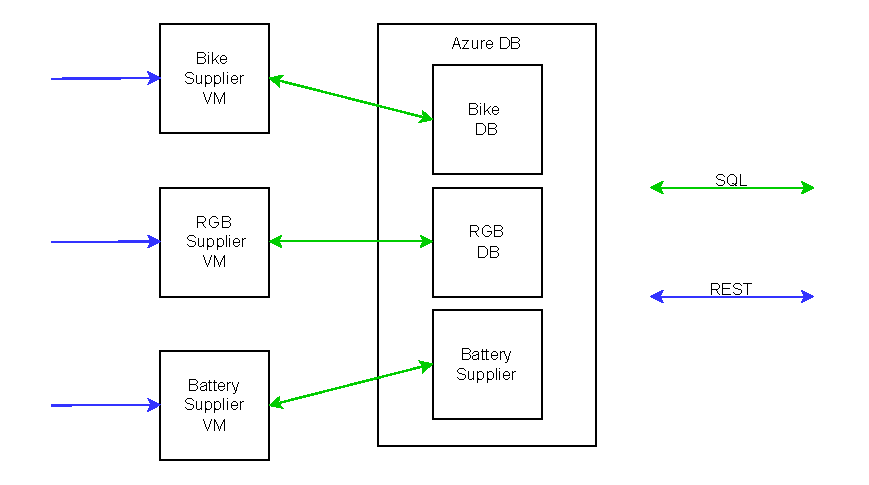
\includegraphics[width=0.7\linewidth]{images/supplier}
				\caption{Detailed architecture of the suppliers}
				\label{fig:supplier}
			\end{figure}
		
	\section{Load testing}
		\subsection{Broker}
			To load test the broker, we added a 1000 orders to the SQL server. Each order consisted of 1 product for every supplier. Next, the Azure Storage Account Queue was instantaneously filled with the order ID`s of these orders. Figure \ref{fig:broker_load} shows the server load of this test. Despite the high number of orders, the server was not greatly affected by this. There was a minimal increase in CPU usage and RAM usage also stayed within limits. This can be explained because, by design, the broker continues to routinely process orders, but the large amount of load is absorbed by the Queue. As a result, it takes a while to fully complete all orders, but the broker itself continues to run smoothly during the whole process. After all orders were completed, we could detect a success rate of 100\% when inspecting the order statuses in the database. We also further examined the effect of an increased number of available threads on the duration of the order processing, but this appeared to have no effect.
			\begin{figure}[h!]
				\centering
				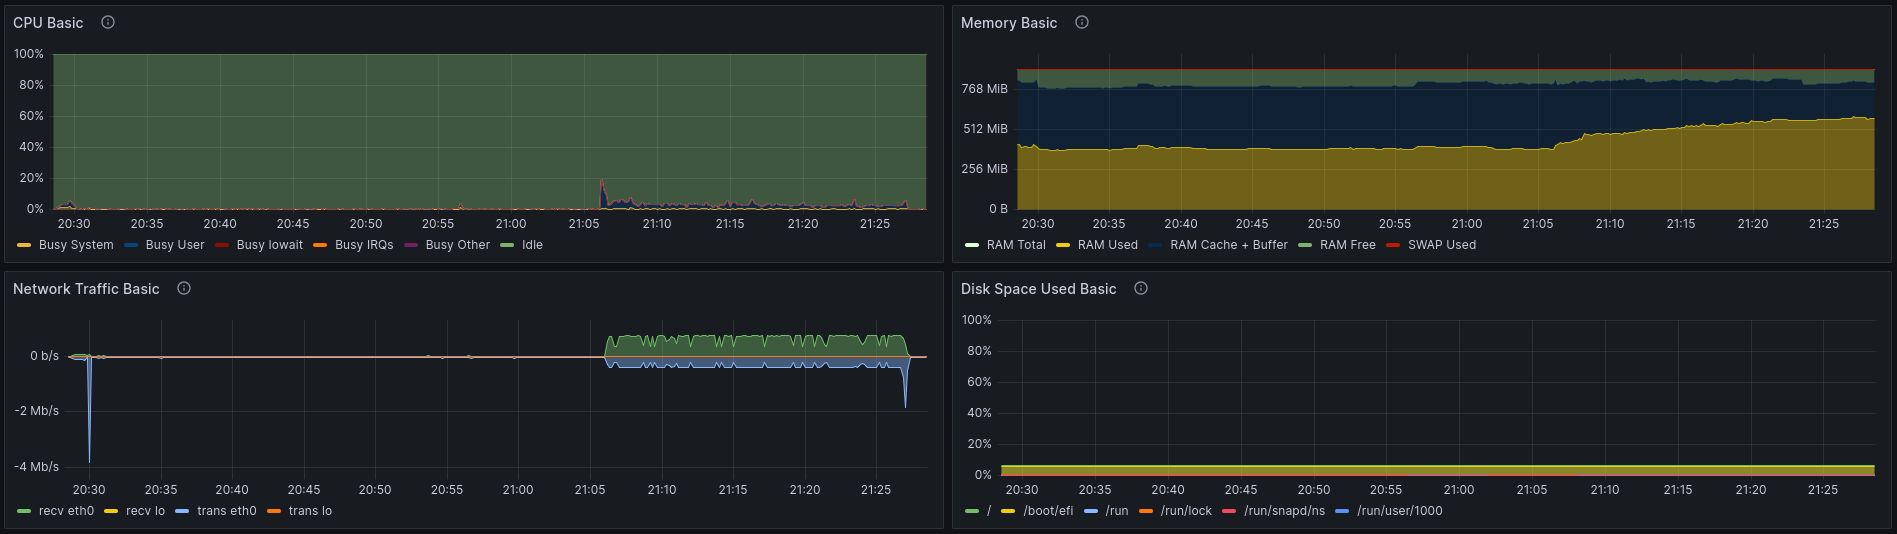
\includegraphics[width=0.9\linewidth]{images/broker-load}
				\caption{Server load on the broker}
				\label{fig:broker_load}
			\end{figure}
		
		\subsection{Suppliers}
			To load test suppliers, we made a script which simulates a full distributed transaction across all three suppliers. This script was run in parallel with 150 instances to load the servers properly. In summary, the load on the servers was lower than expected when running the maximal amount of clients it could handle without returning time-out errors. We suspect the bottleneck is the SQL server which has to handle a lot of queries in order to ensure everything goes smoothly, but further research is needed to confirm this. In the end, with some manual testing of different configurations of the tests, we concluded we could perform about 19 distributed commits per minute. During testing of aborted transactions, we did notice a higher throughput of 55 reverts per minute. This is likely due to the lower overhead required in cancelling a transaction rather than committing it. Performing a synchronisation between suppliers (to simulate a broker crash) did slow down these throughputs a bit, as the mechanism for checking other suppliers has some overhead as well. 
			\begin{figure}[h!]
				\centering
				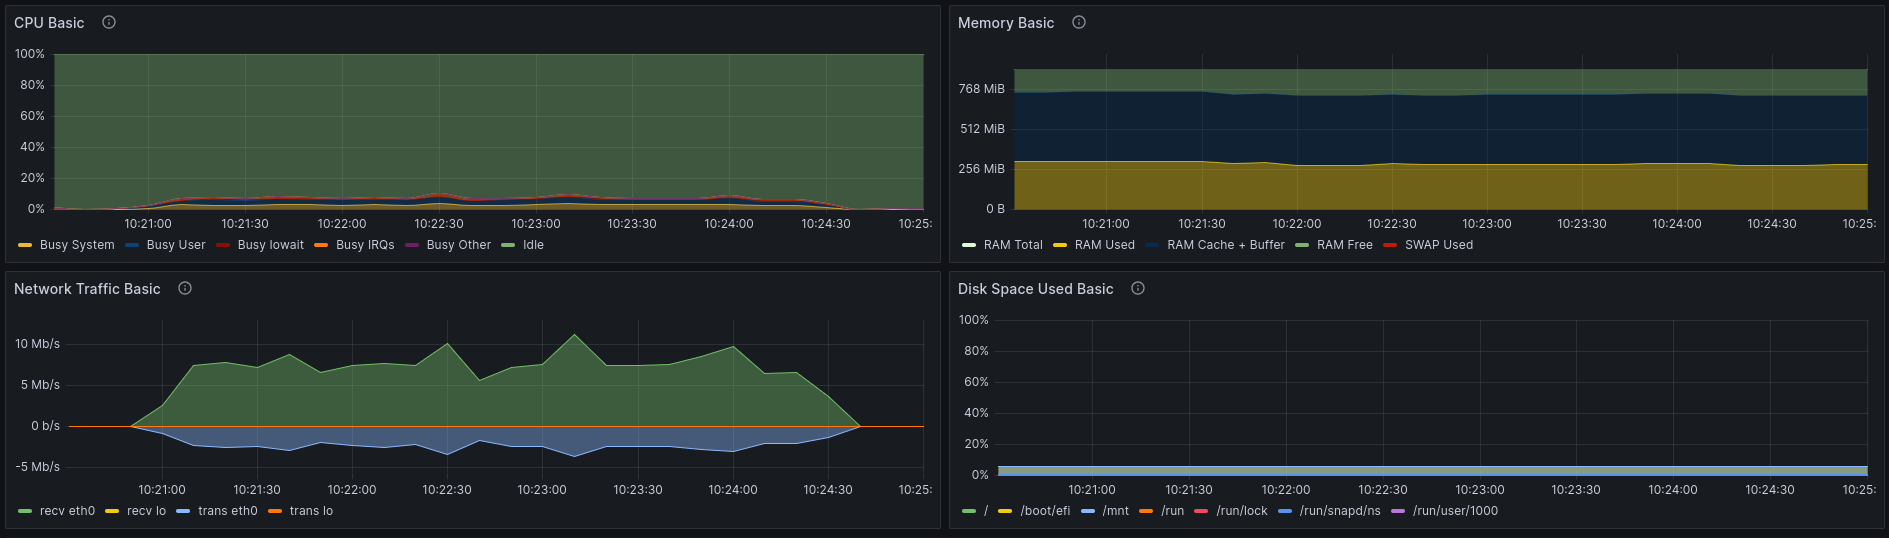
\includegraphics[width=0.9\linewidth]{images/supplier-load}
				\caption{Server load on one of the suppliers}
				\label{fig:supplier_load}
			\end{figure}
			

	\section{Cost overview}
		\subsection{Broker}
			The broker consists of a single Azure virtual machine (VM), an Azure SQL Server and an Azure Storage Queue. All of these instances are operating within cost-conscious constraints. \\		
			The VM on which the Spring Boot broker application is running falls under Azure’s free tier, which offers 750 compute hours per month. If the broker’s usage surpasses this limit, it transitions to Azure’s entry-level paid tier to keep the application running at minimal cost. \\		
			The broker also uses an Azure SQL Server instance to extract and update the order information. Just like the VM, the database operates under Azure’s free tier. This provides 100 000 so-called vCore seconds of serverless database compute and a maximum size of 32 GB of data per database. In case this free limit is reached, the database can be automatically switched to the standard General Purpose tier serverless rates. This results in an additional fee of \$0.0001812 per used vCore-second. \\		
			Finally, the broker communicates asynchronously with the client application using an Azure Storage Queue. This service is not covered by the free tier but is still highly cost-effective. Azure charges \$0.004 per 10 000 operations, which results to negligible cost under typical workloads. Given the brokers polling mechanism where it extracts messages every second, this results in a cost of approximately \$0.035 per day. 
	
		\subsection{Suppliers}
			The supplier infrastructure supporting the web-shop is designed with cost-efficiency in mind, particularly during the initial phases of operation. This infrastructure relies on three virtual machines (VMs) hosted on Microsoft Azure, along with a MySQL database, all of which initially operate within Azure's free tier offerings.\\
			Each of the three VMs benefits from Azure’s free tier, which provides up to 750 compute hours per month. This allocation is sufficient to run one VM continuously or distribute usage across multiple VMs with careful scheduling. Once the 750-hour limit is exceeded in any given billing cycle, the VMs automatically transition to Azure’s lowest-cost paid tier. This tier continues to offer basic compute capabilities at a minimal cost, ensuring that the infrastructure remains economically sustainable even under moderate usage.\\
			Similarly, the MySQL database is provisioned under Azure’s free tier for managed databases. It remains free until it exceeds the usage limits defined by the 750-hour threshold. Upon reaching this limit, the database instance shifts to the lowest available pricing tier, maintaining essential functionality while controlling costs.\\
			By leveraging Azure’s free tier and its seamless transition to cost-effective paid options, the supplier infrastructure is able to support operational demands with minimal upfront expenditure. This approach allows for scalability and consistent performance while keeping cloud resource costs predictable and manageable as usage grows.
	
\newpage
  \section{Extra information}
  \begin{itemize}
    \item Robbe Decapmaker - R0848369
    \item Wout Lyen - R0887788
    \item Lander Van Loock - R0886277
    \item Kobe Michiels - R0848543
  \end{itemize}
  

\end{document}

